\documentclass[a4paper,12pt]{article}

%%% Работа с русским языком % для pdfLatex
\usepackage{cmap}					% поиск в~PDF
\usepackage{mathtext} 				% русские буквы в~фомулах
\usepackage[T2A]{fontenc}			% кодировка
\usepackage[utf8]{inputenc}			% кодировка исходного текста
\usepackage[english,russian]{babel}	% локализация и переносы
\usepackage{indentfirst} 			% отступ 1 абзаца

%%% Работа с русским языком % для XeLatex
%\usepackage[english,russian]{babel}   %% загружает пакет многоязыковой вёрстки
%\usepackage{fontspec}      %% подготавливает загрузку шрифтов Open Type, True Type и др.
%\defaultfontfeatures{Ligatures={TeX},Renderer=Basic}  %% свойства шрифтов по умолчанию
%\setmainfont[Ligatures={TeX,Historic}]{Times New Roman} %% задаёт основной шрифт документа
%\setsansfont{Comic Sans MS}                    %% задаёт шрифт без засечек
%\setmonofont{Courier New}
%\usepackage{indentfirst}
%\frenchspacing

%%% Дополнительная работа с математикой
\usepackage{amsfonts,amssymb,amsthm,mathtools}
\usepackage{amsmath}
\usepackage{icomma} % "Умная" запятая: $0,2$ --- число, $0, 2$ --- перечисление
\usepackage{upgreek}
%\usepackage{mathassents}

%% Номера формул
%\mathtoolsset{showonlyrefs=true} % Показывать номера только у тех формул, на которые есть \eqref{} в~тексте.

%%% Страница
\usepackage{extsizes} % Возможность сделать 14-й шрифт

%% Шрифты
\usepackage{euscript}	 % Шрифт Евклид
\usepackage{mathrsfs} % Красивый матшрифт

%% Свои команды
\DeclareMathOperator{\sgn}{\mathop{sgn}} % создание новой конанды \sgn (типо как \sin)
\usepackage{csquotes} % ещё одна штука для цитат
\newcommand{\pd}[2]{\ensuremath{\cfrac{\partial #1}{\partial #2}}} % частная производная
\newcommand{\abs}[1]{\ensuremath{\left|#1\right|}} % модуль
\renewcommand{\phi}{\ensuremath{\varphi}} % греческая фи
\newcommand{\pogk}[1]{\!\left(\cfrac{\sigma_{#1}}{#1}\right)^{\!\!\!2}\!} % для погрешностей

% Ссылки
\usepackage{color} % подключить пакет color
% выбрать цвета
\definecolor{BlueGreen}{RGB}{49,152,255}
\definecolor{Violet}{RGB}{120,80,120}
% назначить цвета при подключении hyperref
\usepackage[unicode, colorlinks, urlcolor=blue, linkcolor=blue, pagecolor=blue, citecolor=blue]{hyperref} %синие ссылки
%\usepackage[unicode, colorlinks, urlcolor=black, linkcolor=black, pagecolor=black, citecolor=black]{hyperref} % для печати (отключить верхний!)


%% Перенос знаков в~формулах (по Львовскому)
\newcommand*{\hm}[1]{#1\nobreak\discretionary{}
	{\hbox{$\mathsurround=0pt #1$}}{}}

%%% Работа с картинками
\usepackage{graphicx}  % Для вставки рисунков
\graphicspath{{images/}{images2/}}  % папки с картинками
\setlength\fboxsep{3pt} % Отступ рамки \fbox{} от рисунка
\setlength\fboxrule{1pt} % Толщина линий рамки \fbox{}
\usepackage{wrapfig} % Обтекание рисунков и таблиц текстом
\usepackage{multicol}

%%% Работа с таблицами
\usepackage{array,tabularx,tabulary,booktabs} % Дополнительная работа с таблицами
\usepackage{longtable}  % Длинные таблицы
\usepackage{multirow} % Слияние строк в~таблице
\usepackage{caption}
\captionsetup{labelsep=period, labelfont=bf}

%%% Оформление
\usepackage{indentfirst} % Красная строка
%\setlength{\parskip}{0.3cm} % отступы между абзацами
%%% Название разделов
\usepackage{titlesec}
\titlelabel{\thetitle.\quad}
\renewcommand{\figurename}{\textbf{Рис.}}		%Чтобы вместо figure под рисунками писал "рис"
\renewcommand{\tablename}{\textbf{Таблица}}		%Чтобы вместо table над таблицами писал Таблица

%%% Теоремы
\theoremstyle{plain} % Это стиль по умолчанию, его можно не переопределять.
\newtheorem{theorem}{Теорема}[section]
\newtheorem{proposition}[theorem]{Утверждение}

\theoremstyle{definition} % "Определение"
\newtheorem{definition}{Определение}[section]
\newtheorem{corollary}{Следствие}[theorem]
\newtheorem{problem}{Задача}[section]

\theoremstyle{remark} % "Примечание"
\newtheorem*{nonum}{Решение}
\newtheorem{zamech}{Замечание}[theorem]

%%% Правильные мат. символы для русского языка
\renewcommand{\epsilon}{\ensuremath{\varepsilon}}
\renewcommand{\phi}{\ensuremath{\varphi}}
\renewcommand{\kappa}{\ensuremath{\varkappa}}
\renewcommand{\le}{\ensuremath{\leqslant}}
\renewcommand{\leq}{\ensuremath{\leqslant}}
\renewcommand{\ge}{\ensuremath{\geqslant}}
\renewcommand{\geq}{\ensuremath{\geqslant}}
\renewcommand{\emptyset}{\varnothing}

\usepackage{bm} %жирный греческий шрифт
%\usepackage{ulem}

\graphicspath{{images}}


\usepackage{graphicx,xcolor,adjustbox,setspace, amsmath,pdfpages}

\newcommand{\resh}{\noindent\textit{Решение:}\\}

\newcounter{prim}
\newenvironment{prim}{%
	\addtocounter{prim}{1}
	\noindent{\\
		\textbf{\noindentПример \arabic{prim}\\}}%
}{\vspace{2mm}\\
\resh
}
\definecolor{orange}{rgb}{1, 0.7, 0.1}
%\usepackage{ulem}

\usepackage{bm} %жирный греческий шрифт

\newenvironment{psm}
{\left(\begin{smallmatrix*}[r]}
	{\end{smallmatrix*}\right)}

\newenvironment{pmatrixr}
{\begin{pmatrix*}[r]}
	{\end{pmatrix*}}

\newenvironment{solution}{%
    \textbf{Решение}%
}

\renewcommand{\figurename}{\textbf{Рис.}}		%Чтобы вместо figure под рисунками писал "рис"
\renewcommand{\tablename}{\textbf{Таблица}}		%Чтобы вместо table над таблицами писал Таблица


\title{ans2014}
\author{Кожарин Алексей}
\date{Nov 2021}
\usepackage[left=1.27cm,right=1.27cm,top=1.27cm,bottom=2cm]{geometry}

\begin{document}
	
\section{Задача №921}

    \subsection{Условие}
    Найти все положения равновесия и исследовать их на устойчивость.
    Решить тремя способами:
    \begin{itemize}
        \item Через характеристический многочлен;
        \item Через критерий Гурвица;
        \item Через критерий Михайлова.
    \end{itemize}

    \begin{equation}
        \begin{cases}
            \dot x = \ln (1 + y + \sin x) \\
        \dot y = 2 + (3 \sin x - 8)^{\frac{1}{3}}
        \end{cases}
    \end{equation}

    \subsection{Решение}
    Система уравнений
    \begin{equation}
        \begin{cases}
            0 = \ln (1 + y + \sin x) \\
            0 = 2 + (3 \sin x - 8)^{\frac{1}{3}}
        \end{cases}
    \end{equation}

    из второго уравнения получим $3 \sin x - 8 = -8 \Leftrightarrow x = k \pi, k \in \mathbb{Z}$, а после подстановки во второе имеем $ y = 0$.
    Итого система имеет следующие пары действительных корней: $(k \pi, 0)$, где $k \in \mathbb{Z}$.

    Делаем замену: $x = k\pi + \epsilon_1,\, y=\epsilon_2$ и проводим разложение до линейных членов (с учетом $\sin (k\pi + x) = (-1)^k \sin x$), что дает:
    \begin{equation}
        \begin{cases}
            \dot \epsilon_1 = \epsilon_2 + (-1)^k\, \epsilon_1 \\
            \dot \epsilon_2 = \frac{1}{4}\,(-1)^k\,\epsilon_1
        \end{cases}
    \end{equation}

    Этому соответствует характеристический многочлен:

    \begin{equation}
        \lambda^2 + (-1)^{k+1}\lambda + \frac{1}{4}\, (-1)^{k+1}
        \label{eq:char_polyn}
    \end{equation}
    \subsubsection{Характеристический многочлен}
    Корнями характеристического многочлена являются $\lambda_{1,2} = \cfrac{1}{2} \left((-1)^k \pm \sqrt{1 + (-1)^k} \right)$.
    При $k = 2n + 1, n \in \mathbb{N}$ имеем $\mathrm{Re}\, \lambda_{1, 2} < 0$.
    Следовательно, точки равновесия $((2n + 1)\pi, 0)$ \textbf{устойчивы}.
    Если же $k = 2n$, то $\mathrm{Re}\, \lambda_1 > 0$.
    Следовательно, точки равновесия $(2n\pi, 0)$ \textbf{неустойчивы}.
    \subsubsection{Критерий Гурвица}
    Матрица Гурвица
    \[
    \Delta = \begin{bmatrix}
        (-1)^{k+1} & 0 \\
        1 & \cfrac{1}{4}\, (-1)^{k+1}
    \end{bmatrix}
    \]

    Первый минор положителен тогда и только тогда, когда $k = 2n + 1, n \in \mathbb{Z}$.
    При этих $k$ будет положителен второй минор и свободный член.
    При $k = 2n$ оба минора отрицательны и отрицателен свободный член.

    Следовательно, по критерию Гурвица точки равновесия $((2n+1)\pi, 0)$ \textbf{устойчивы}, а точки $(2n\pi, 0)$ -- \textbf{неустойчивы}.

    \subsubsection{Критерий Михайлова}
    Уравнение характеристической кривой:
    \begin{equation}
        D(i\omega) = -\omega^2 + (-1)^{k+1}\, i \omega + \frac{1}{4}\, (-1)^{k+1}
        \label{eq:mihalich}
    \end{equation}

    Для $\omega \rightarrow 0$ при $k = 2n+1$ имеем $\arg D (i \omega) \rightarrow 0$, при $k = 2n$ имеем $\arg D(i\omega) \rightarrow \pi$.

    Для $\omega \rightarrow +\infty$ получим $\arg D(i\omega) \rightarrow \pi$.

    По критерию Михайлова, для устойчивости системы необходимо и достаточно, чтобы вектор кривой Михайлова $D (i\omega)$ при изменении частоты $\omega$ от $0$ до $+\infty$ повернулся, нигде не обращаясь в нуль, вокруг начала координат против часовой стрелки на угол $n \pi / 2$, где $n$ обозначает порядок характеристического уравнения.

    В случае $k = 2n+1$ вектор повернется на $\pi = \frac{2}{2}\,\pi$ против часовой стрелки, нигде не обращаясь в нуль (т.к. присутствует свободный член). Следовательно, по критерию Михайлова точки ${((2n+1)\pi,~0)}$ \textbf{устойчивы}.

    В случае $k = 2n$ вектор повернется на $0 \neq \frac{2}{2}\,\pi$, нигде не обращаясь в нуль. Следовательно, по критерию Михайлова точки $(2n\pi,~0)$ \textbf{не устойчивы}.

    В целях иллюстрации приведем качественный вид кривой Михайлова.

    \begin{figure}[h]
        \caption{Кривая Михайлова}
        \centering
        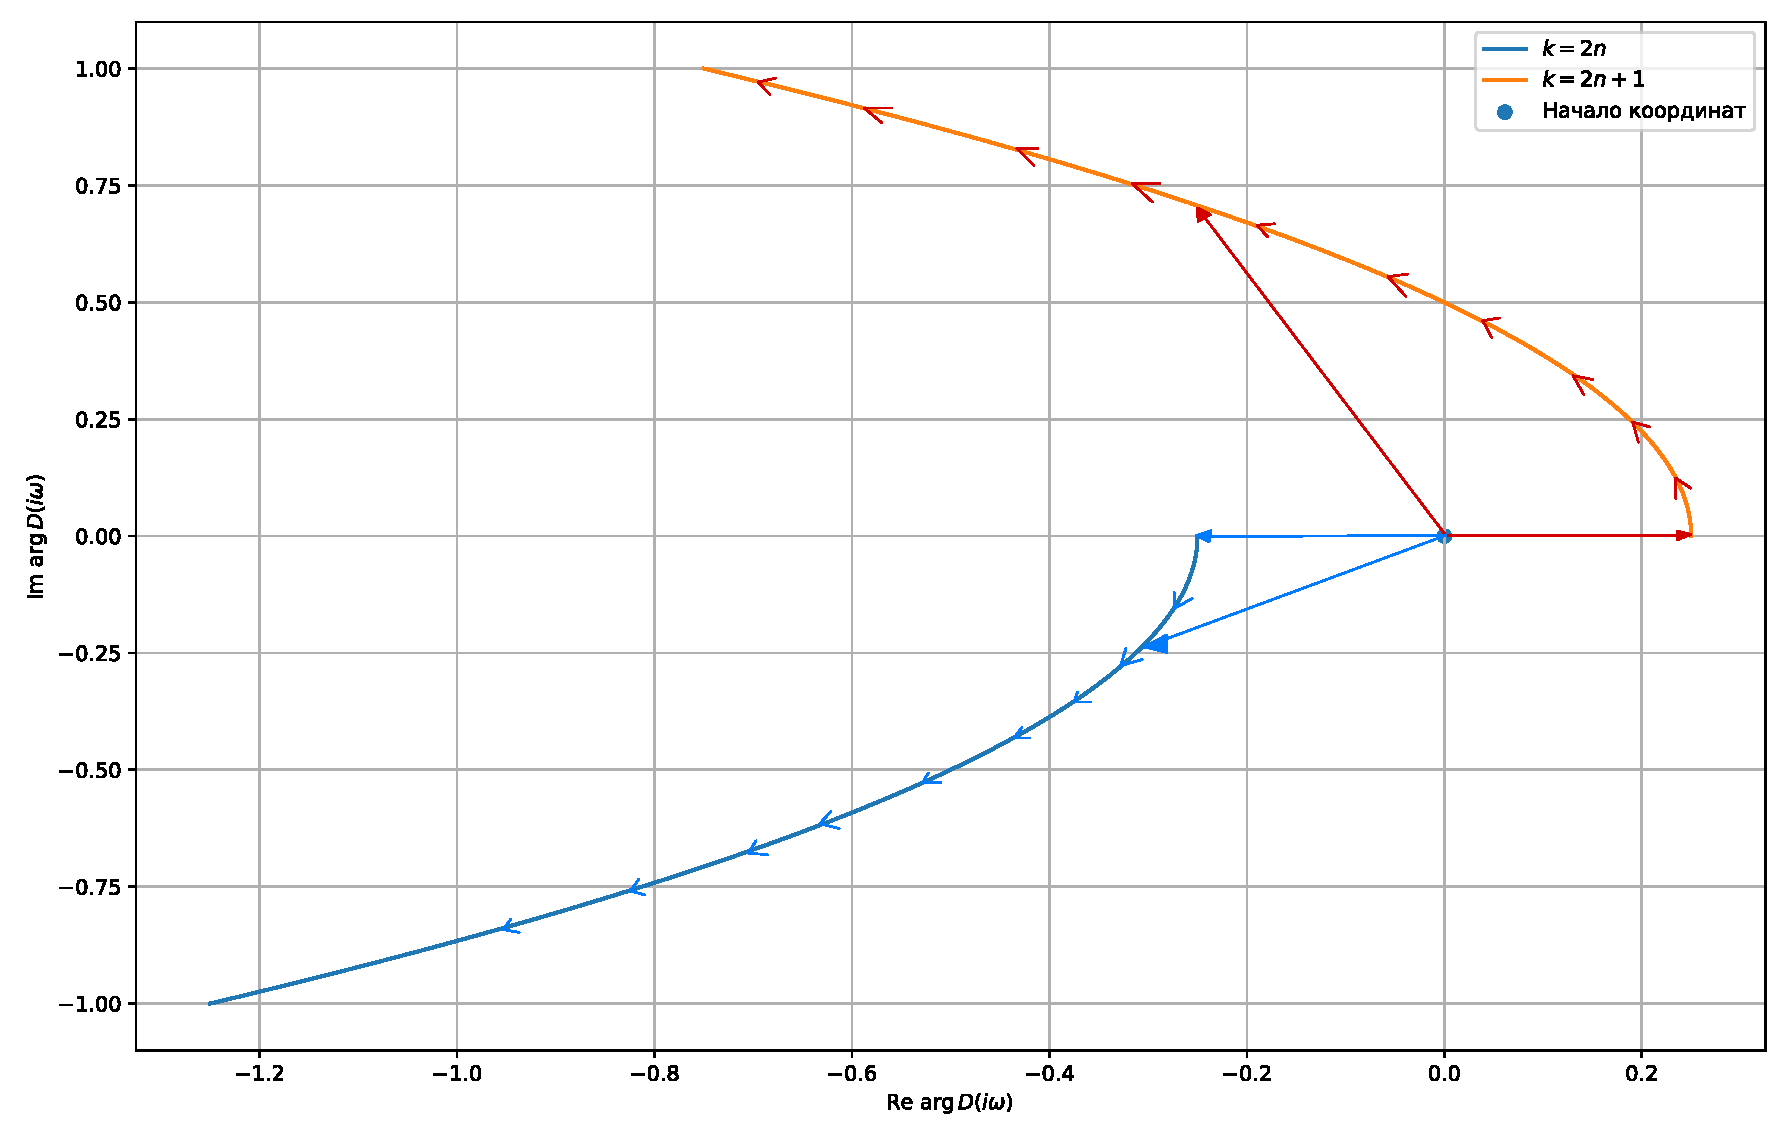
\includegraphics[width=\textwidth]{mih.pdf}
    \end{figure}

    На рисунке стреками вдоль графика обозначен ход кривой при увеличении $\omega$ от $0$ до $+\infty$.
    Векторы, проведенные из начала координат, иллюстрируют изменение угла при увеличении $\omega$ от $0$ в сторону $+\infty$.
    Синяя линия <<начинается>> с аргумента $\phi = \pi$ и при $\omega \rightarrow +\infty$ стремится к $\phi = \pi$, при этом $\forall \omega$ выполнено $\phi \in [\pi, \frac{3}{2}\,\pi)$. Это дает изменение аргумента, равное $0$.

    Оранжевая линия <<начинается>> с аргумента $\phi = 0$ и при $\omega \rightarrow +\infty$ стремится к $\phi = \pi$, что дает изменение аргумента, равное $\pi$.

\end{document}
